\chapter{概述}

本章介绍课程管理系统的项目背景并简要阐述 Model-View-ViewModel (MVVM) 模式、Functional Reactive Programming (FRP) 方法的核心思想及特性。

\section{项目背景}

用户交互(User Interaction)在消费级产品开发中的地位近年来正不断提升,交互设计和实现正成为产品开发中最重要也最复杂的环节之一。随着互联网的发展、富交互应用(Rich Interaction Application, RIA)的兴起,交互设计正走向越来越复杂的方向。使用传统的命令式编程(Imperative Programming)实现用户交互逻辑的局限性也不断显现出来。

Microsoft 在 Windows Presentation Framework (WPF) 中引入的 Model-View-ViewModel(MVVM) 模式近年来得到了相当广泛的关注和应用~\footnote{Wikipedia: Model View ViewModel}。MVVM模式作为如今最成功的图形用户界面(Graphical User Interface, GUI)开发模式之一,将声明式方法引入用户交互开发,解决了命令式编程方法在处理异步逻辑时难于维持代码逻辑连续性的问题。

课程管理系统作为面向业务产品的典型代表,工程规模足够体现设计模式的各项性能。本文以课程管理产品的设计与开发为线索,尝试解释 MVVM 设计模式的设计方法,并从 FRP 的角度解释 MVVM 模式中 ViewModel 部分的设计,在此基础上使用 monad 结构~\cite{raey}开发 MVVM 框架并测试该框架在课程管理系统中实际进行富交互应用开发的性能。

\section{Model-View-ViewModel~模式}

经典的 MVC 模式~\footnote{Wikipedia: Model–view–controller} 将系统分成 Model(模型)、View(视图)、Controller(控制器) 三个部分: Model 对象用于处理数据和业务操作、View 对象控制视图逻辑、Controller 负责处理用户操作。MVC 架构作为许多互联网产品和应用的基础架构在各大开发平台都有成熟的解决方案和技术框架~\footnote{如 Ruby-on-Rails、ThinkMVC 等广泛应用的 Web 框架都基于 MVC 架构进行开发}。

\begin{figure}[!h]
\begin{center}
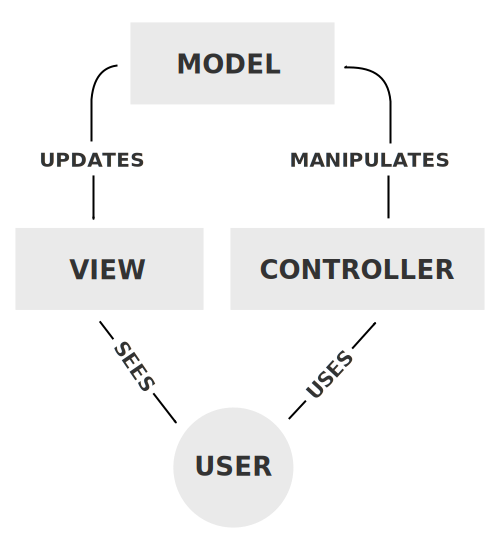
\includegraphics[scale=0.5]{figures/pattern-mvc.pdf}
\caption{MVC 模式\label{MVCOverview}}
\end{center}
\end{figure}

Microsoft 作为用户交互领域的先驱,最早在 2005 年由工程师 Martin Fowler 提出了 MVVM 架构并应用于 Windows Presentation Framework。

\begin{figure}[!h]
\begin{center}
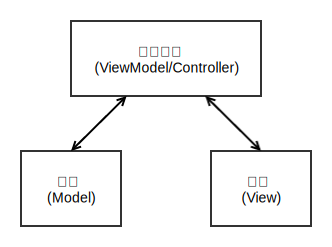
\includegraphics[scale=0.7]{figures/pattern-mvvm.pdf}
\caption{MVVM 模式\label{MVVMOverview}}
\end{center}
\end{figure}

Model-View-ViewModel (MVVM) 模式是 Model-View-Controller (MVC) 模式的一种特化(见图~\ref{MVVMOverview}): MVC 模式中 Controller 负责进行的界面业务逻辑部分抽象为 ViewModel 以及 Binder 组合。一方面利用 ViewModel 管理交互状态、另一方面通过 Binder 将状态通过 View 进行展示。用户产生的交互事件也经由 Binder 传递至 ViewModel 对用户界面的状态以及 Model 状态产生影响。

MVVM 模式的一大设计亮点在于“ViewModel 继承于 Model” 即: ViewModel 可以将另一个 ViewModel 实例作为 Model 进行数据请求。这是 ViewModel 与 Controller 之间最大的不同,也是 ViewModel 较 Controller 实现拥有更高的可复用性以及更良好的可测试性的原因。

另外,MVVM 模式解除了 Controller 代码与视图实现之间的耦合关系,界面设计人员仅需要在XAML(对WPF的情况)文档中描述视图对象所需要绑定(bind)的数据位置(属性名称)即可完成用户交互设计任务,而在 MVC 模式中设计者需要书写 Controller 代码以描述视图对象所需要的呈现数据。

MVVM 模式在普遍用于用户交互开发的 JavaScript 语言中也得到了类似的实现,如 AngularJS、KnockoutJS 等开发框架。

\section{Functional Reactive Programming (FRP)}

Functional Reactive Programming (FRP) 是使用声明式 (Declarative) 方法描述系统行为的编程方法。FRP 的主要思想是将系统抽象为 $行为(Behaviors)$ 和 $事件(Events)$,使用行为表示系统中随时域连续变化的值、事件表示一系列按一定时序触发的离散值~\cite{Wan:2000:FRP:358438.349331}。最初,FRP 方法被应用于 Haskell 的 Functional Reactive Animation (Fran) 的核心实现~\cite{Elliott:1997:FRA:258949.258973}。后来,FRP 方法被广泛的用于计算机视觉、机器人以及其他控制系统的设计和实现。

简而言之,FRP 抽象系统为用户与函数(Behavior)的交互,用户事件作为函数的自变量,而模型/用户视图作为函数作用的因变量。

随着 FRP 理论的成熟与富交互应用的发展,FRP 的影响也逐渐延伸到应用开发的前沿领域,出现了许多成熟的 FRP 开发框架,如 Objective C 平台下的 ReactiveCocoa,.NET Framework 下的 ReactiveUI 以及 JavaScript 平台下的 Reactive.js 等~\footnote{虽然这些框架是实现在命令式语言平台的 Reactive Programming 框架,这里还是沿用 Haskell 中 FRP 的名称}。

FRP 方法与 MVVM 使用的 Observer 模式具有很高的相似性,本文将在后面的章节围绕此问题进行一番讨论并提出作者对 MVVM 架构模式的理解。

后文分成五个部分: 第二章、第三章分别介绍系统的需求分析和概要设计,第四章引入有关MVVM模式与 Reactive Programming 的讨论、描述 ReactiveVM 的设计思路,第五章讨论实现过程中出现的探索性过程,第六章对项目的开发过程进行一个总结并描述一下对未来研究方向的展望。

